\documentclass[stu,biblatex,floatsintext,draftall]{apa7}

\usepackage{graphicx}
\graphicspath{{assets/}}

\usepackage{siunitx}
\usepackage{multirow}

\addbibresource{refs.bib}

\title{Investigating the Effect of Chain Length on Change in Acceleration}
\author{Adam Zhang}
\affiliation{Academies of Loudoun}
\course{AP Physics C: Mech, Block 2}
\professor{Matthew Hilsdorf}
\duedate{September 21 2023}

\begin{document}
\maketitle
\tableofcontents
\newpage

\section{Introduction}

\subsection{Purpose}
Investigate the effect of the length of a heavy chain on the rate of change of the acceleration (jerk) of the chain as it falls off a pulley.

\subsection{Hypothesis}
An increase in the length of the chain will result in an increase in the rate of change of acceleration (jerk) of the chain.

\subsection{Background}
Describe relevant background, concepts, and applicable equations, with citations.

\section{Methods}

\subsection{Materials}
The following materials are required for this experiment \parencite{Hilsdorf2023AtwoodsHeavyChainHandout}:
\begin{APAitemize}
	% TODO Add links and symbols
	\item Vernier ultra pulley (green)
	\item Vernier photogate and connection cable
	\item Vernier LabQuest
	\item Meter stick
	\item Chains of varying lengths % TODO clarify
\end{APAitemize}
The setup of the experiment is shown in Figure \ref{fig:setup}.
\begin{figure}
	\centering
	\caption{Experimental Setup}
	\label{fig:setup}
	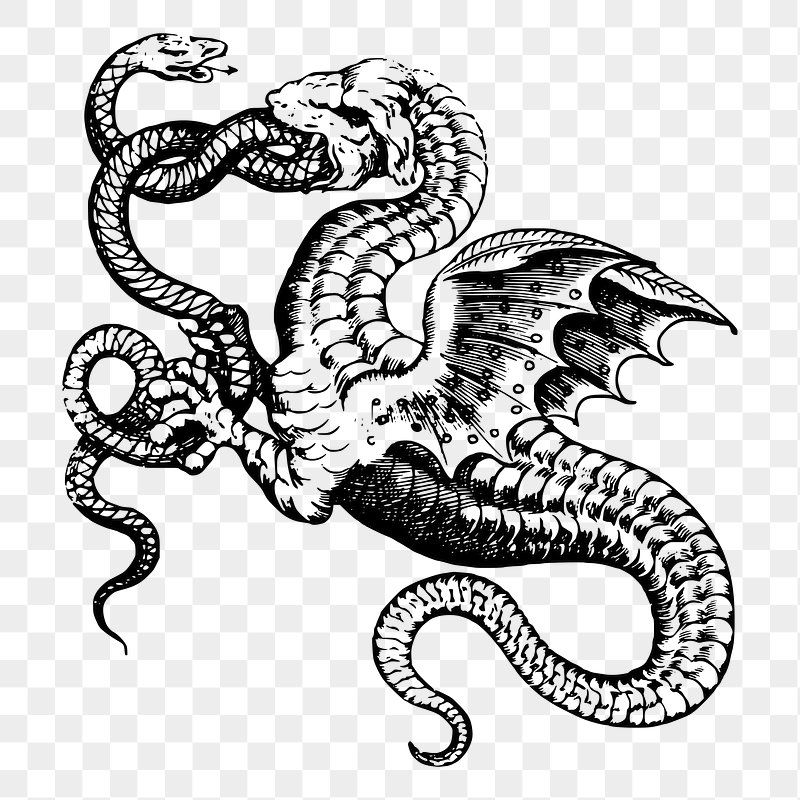
\includegraphics{dragon}
\end{figure}

\subsection{Procedures}
The following procedure was implemented during this experiment.
\begin{APAenumerate}
	\item Construct the experimental setup as shown in Figure \ref{fig:setup}.
	\item\label{pro:outer-start} Place the 60\unit{\centi\meter} chain on the pulley so that 25\unit{\centi\meter} of the chain is on the side away from the photogate.
	\item\label{pro:inner-start} Start collecting data on the LabQuest, then release the chain.
	\item\label{pro:inner-end} End the data collection after the chain has fallen.
	\item\label{pro:outer-end} Repeat steps \ref{pro:inner-start} through \ref{pro:inner-end} two more times to obtain 3 total trials for this length.
	\item Repeat steps \ref{pro:outer-start} through \ref{pro:outer-end} four more times, increasing the chain length by 10\unit{\centi\meter} every time to obtain a total of 15 trials.
\end{APAenumerate}

\section{Results}

\subsection{Data}
For each trial, a trend line was fitted to the velocity data points. The equation of this velocity line is shown in Table \ref{tab:equations}. An example graph for the first trial of the 100\unit{\centi\meter} chain is shown in Figure \ref{fig:100-trial1}. For completeness, the distance and interpolated acceleration is included in the graph.

\begin{table}
	\centering
	\caption{Trend Line Equations for Each Trial}
	\label{tab:equations}
	\begin{tabular}{|c|c|c|}
		\hline
		Chain Length (\unit{\centi\meter}) & Trial \# & Velocity Equation ($v(t)$) \\
		\hline
		\multirow{3}{*}{60\unit{\centi\meter} Chain}
		& 1 & $0.145e^{5.022t}$ \\
		& 2 & $0.102e^{5.116t}$ \\
		& 3 & $0.105e^{5.107t}$ \\
		\hline
		\multirow{3}{*}{70\unit{\centi\meter} Chain}
		& 1 & $0.180e^{5.164t}$ \\
		& 2 & $0.205e^{5.238t}$ \\
		& 3 & $0.205e^{5.370t}$ \\
		\hline
		\multirow{3}{*}{80\unit{\centi\meter} Chain}
		& 1 & $0.135e^{5.183t}$ \\
		& 2 & $0.351e^{4.602t}$ \\
		& 3 & $0.116e^{5.548t}$ \\
		\hline
		\multirow{3}{*}{90\unit{\centi\meter} Chain}
		& 1 & $0.177e^{5.306t}$ \\
		& 2 & $0.334e^{5.046t}$ \\
		& 3 & $0.336e^{5.197t}$ \\
		\hline
		\multirow{3}{*}{100\unit{\centi\meter} Chain}
		& 1 & $0.436e^{4.922t}$ \\
		& 2 & $0.201e^{5.931t}$ \\
		& 3 & $0.344e^{5.398t}$ \\
		\hline
	\end{tabular}
\end{table}
\begin{figure}[H]
	\centering
	\caption{Graph for First Trial of 100\unit{\centi\meter} Chain}
	\label{fig:100-trial1}
	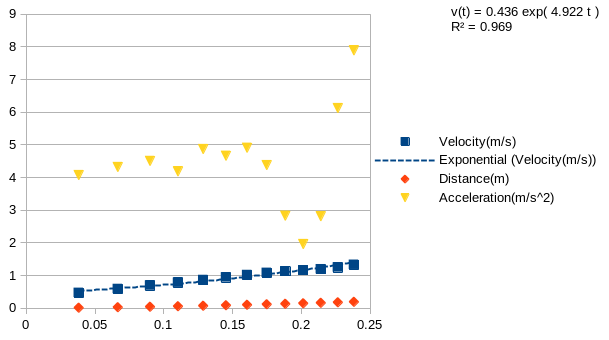
\includegraphics[width=0.75\textwidth]{100-trial1}
\end{figure}

\subsection{Calculations}
% TODO explain calculations
The calculated equation for acceleration for each trial is shown in Table \ref{tab:acceleration-equation}. The constant for rate of growth for each trial, as well as an average, is shown in Table \ref{tab:acceleration-rog}. A scatterplot of the average rate of growth per chain length is shown in Figure [?]. % TODO

\begin{table}
	\centering
	\caption{Equation and Rate of Growth for Acceleration per Trial}
	\label{tab:acceleration-equation}
	\begin{tabular}{|c|c|c|c|}
    	\hline
		Chain Length (\unit{\centi\meter}) & Trial \# & Acceleration Equation ($a(t)$) \\
		\hline
		\multirow{3}{*}{60\unit{\centi\meter} Chain}
		& 1 & $0.728e^{5.022t}$ \\ 
		\cline{2-3}
		& 2 & $0.523e^{5.116t}$ \\
		\cline{2-3}
		& 3 & $2.666e^{5.107t}$ \\
		\hline
		\multirow{3}{*}{70\unit{\centi\meter} Chain}
		& 1 & $0.930e^{5.164t}$ \\
		\cline{2-3}
		& 2 & $1.074e^{5.238t}$ \\
		\cline{2-3}
		& 3 & $1.101e^{5.370t}$ \\
		\hline
		\multirow{3}{*}{80\unit{\centi\meter} Chain}
		& 1 & $0.700e^{5.183t}$ \\
		\cline{2-3}
		& 2 & $1.615e^{4.602t}$ \\
		\cline{2-3}
		& 3 & $0.644e^{5.548t}$ \\
		\hline
		\multirow{3}{*}{90\unit{\centi\meter} Chain}
		& 1 & $0.939e^{5.306t}$ \\
		\cline{2-3}
		& 2 & $1.685e^{5.046t}$ \\
		\cline{2-3}
		& 3 & $1.746e^{5.197t}$ \\
		\hline
		\multirow{3}{*}{100\unit{\centi\meter} Chain}
		& 1 & $2.146e^{4.922t}$ \\
		\cline{2-3}
		& 2 & $1.192e^{5.931t}$ \\
		\cline{2-3}
		& 3 & $1.857e^{5.398t}$ \\
		\hline
    \end{tabular}
\end{table}

\begin{table}[H]
	\centering
	\caption{Rate of Growth of Acceleration}
	\label{tab:acceleration-rog}
	\begin{tabular}{|c|c|c|c|}
    	\hline
		Chain Length (\unit{\centi\meter}) & Trial \# & Rate of Growth & Average \\
		\hline
		\multirow{3}{*}{60\unit{\centi\meter} Chain} & 1 & 5.022 & \multirow{3}{*}{5.082} \\
		\cline{2-3}
		& 2 & 5.116 & \\
		\cline{2-3}
		& 3 & 5.107 & \\
		\hline
		\multirow{3}{*}{70\unit{\centi\meter} Chain} & 1 & 5.164 & \multirow{3}{*}{5.257} \\
		\cline{2-3}
		& 2 & 5.238 & \\
		\cline{2-3}
		& 3 & 5.370 & \\
		\hline
		\multirow{3}{*}{80\unit{\centi\meter} Chain} & 1 & 5.183 & \multirow{3}{*}{5.111} \\
		\cline{2-3}
		& 2 & 4.602 & \\
		\cline{2-3}
		& 3 & 5.548 & \\
		\hline
		\multirow{3}{*}{90\unit{\centi\meter} Chain} & 1 & 5.306 & \multirow{3}{*}{5.183} \\
		\cline{2-3}
		& 2 & 5.046 & \\
		\cline{2-3}
		& 3 & 5.197 & \\
		\hline
		\multirow{3}{*}{100\unit{\centi\meter} Chain} & 1 & 4.922 & \multirow{3}{*}{5.417} \\
		\cline{2-3}
		& 2 & 5.931 & \\
		\cline{2-3}
		& 3 & 5.398 & \\
		\hline
    \end{tabular}
\end{table}

\section{Discussion}

\subsection{Conclusion}
Discuss if the hypothesis was satisfied, including data/evidence from experiment. Reflect on the success/failure of the experiment (purpose accomplished or not). Make a claim, support it with evidence from the experiment, and use reasoning related to the principles discussed in the background to support it.

\subsection{Errors}
Describe errors and sources of error. Be specific. Comment on the percent error calculation (if applicable).  Include a discussion of how to minimize error in further research. 

\subsection{Extensions}
Explain how the conclusions and experiment are relevant to real-life.  Provide commentary to answer required questions.

\printbibliography

\end{document}
